\documentclass{standalone}
\usepackage{tikz}
\usetikzlibrary{patterns, positioning}


\begin{document}
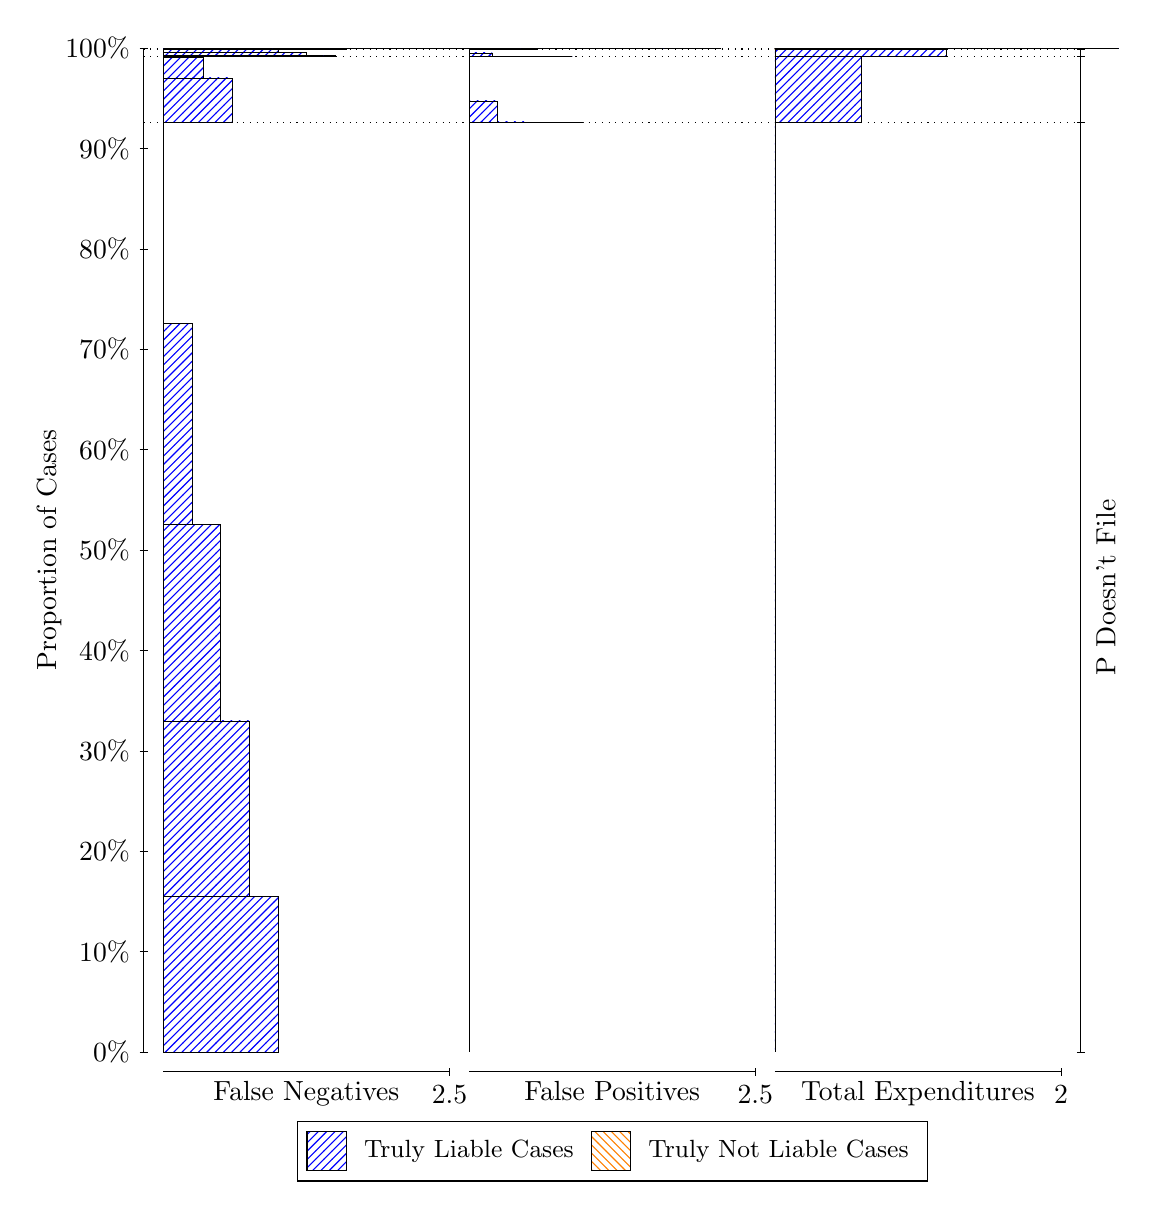
\begin{tikzpicture}
\draw[black, very thin] (1.5,1.75) -- (1.5,14.5);
\node[rotate=90, text=black, anchor=center] at (0.3, 8.125) {Proportion of Cases};
\draw[black, very thin] (1.45,1.75) -- (1.55,1.75);
\node[text=black, anchor=east] at (1.45, 1.75) {0\%};
\draw[black, very thin] (1.45,3.025) -- (1.55,3.025);
\node[text=black, anchor=east] at (1.45, 3.025) {10\%};
\draw[black, very thin] (1.45,4.3) -- (1.55,4.3);
\node[text=black, anchor=east] at (1.45, 4.3) {20\%};
\draw[black, very thin] (1.45,5.575) -- (1.55,5.575);
\node[text=black, anchor=east] at (1.45, 5.575) {30\%};
\draw[black, very thin] (1.45,6.85) -- (1.55,6.85);
\node[text=black, anchor=east] at (1.45, 6.85) {40\%};
\draw[black, very thin] (1.45,8.125) -- (1.55,8.125);
\node[text=black, anchor=east] at (1.45, 8.125) {50\%};
\draw[black, very thin] (1.45,9.4) -- (1.55,9.4);
\node[text=black, anchor=east] at (1.45, 9.4) {60\%};
\draw[black, very thin] (1.45,10.675) -- (1.55,10.675);
\node[text=black, anchor=east] at (1.45, 10.675) {70\%};
\draw[black, very thin] (1.45,11.95) -- (1.55,11.95);
\node[text=black, anchor=east] at (1.45, 11.95) {80\%};
\draw[black, very thin] (1.45,13.225) -- (1.55,13.225);
\node[text=black, anchor=east] at (1.45, 13.225) {90\%};
\draw[black, very thin] (1.45,14.5) -- (1.55,14.5);
\node[text=black, anchor=east] at (1.45, 14.5) {100\%};

\draw[black, very thin] (13.4,1.75) -- (13.4,14.5);
\draw[black, very thin] (13.35,1.75) -- (13.45,1.75);
\node[anchor=west] at (13.35, 1.75) {};
\draw[black, very thin] (13.35,13.553) -- (13.45,13.553);
\node[anchor=west] at (13.35, 13.553) {};
\draw[black, very thin] (13.35,14.396) -- (13.45,14.396);
\node[anchor=west] at (13.35, 14.396) {};
\draw[black, very thin] (13.35,14.485) -- (13.45,14.485);
\node[anchor=west] at (13.35, 14.485) {};
\draw[black, very thin] (13.35,14.493) -- (13.45,14.493);
\node[anchor=west] at (13.35, 14.493) {};
\draw[black, very thin] (13.35,14.498) -- (13.45,14.498);
\node[anchor=west] at (13.35, 14.498) {};
\draw[black, very thin] (13.35,14.5) -- (13.45,14.5);
\node[anchor=west] at (13.35, 14.5) {};

\draw[black, very thin, pattern color=blue, pattern=north east lines] (1.75,1.75) rectangle (3.2033,3.7231);
\draw[black, very thin, pattern color=blue, pattern=north east lines] (1.75,3.7231) rectangle (2.84,5.9548);
\draw[black, very thin, pattern color=blue, pattern=north east lines] (1.75,5.9548) rectangle (2.4767,8.4538);
\draw[black, very thin, pattern color=blue, pattern=north east lines] (1.75,8.4538) rectangle (2.1133,11.003);
\draw[black, very thin, pattern color=orange, pattern=north west lines] (1.75,11.003) rectangle (1.75,11.003);
\draw[black, very thin, pattern color=blue, pattern=north east lines] (1.75,11.003) rectangle (1.75,13.553);
\draw[black, very thin, pattern color=blue, pattern=north east lines] (1.75,13.553) rectangle (2.622,14.122);
\draw[black, very thin, pattern color=blue, pattern=north east lines] (1.75,14.122) rectangle (2.2587,14.388);
\draw[black, very thin, pattern color=blue, pattern=north east lines] (1.75,14.388) rectangle (1.8953,14.396);
\draw[black, very thin, pattern color=orange, pattern=north west lines] (1.75,14.396) rectangle (1.75,14.396);
\draw[black, very thin, pattern color=blue, pattern=north east lines] (1.75,14.396) rectangle (1.75,14.396);
\draw[black, very thin, pattern color=blue, pattern=north east lines] (1.75,14.396) rectangle (3.93,14.402);
\draw[black, very thin, pattern color=blue, pattern=north east lines] (1.75,14.402) rectangle (3.7847,14.402);
\draw[black, very thin, pattern color=blue, pattern=north east lines] (1.75,14.402) rectangle (3.6393,14.402);
\draw[black, very thin, pattern color=blue, pattern=north east lines] (1.75,14.402) rectangle (3.5667,14.442);
\draw[black, very thin, pattern color=blue, pattern=north east lines] (1.75,14.442) rectangle (3.4213,14.443);
\draw[black, very thin, pattern color=blue, pattern=north east lines] (1.75,14.443) rectangle (3.276,14.443);
\draw[black, very thin, pattern color=blue, pattern=north east lines] (1.75,14.443) rectangle (3.2033,14.484);
\draw[black, very thin, pattern color=blue, pattern=north east lines] (1.75,14.484) rectangle (3.058,14.484);
\draw[black, very thin, pattern color=blue, pattern=north east lines] (1.75,14.484) rectangle (2.9127,14.484);
\draw[black, very thin, pattern color=blue, pattern=north east lines] (1.75,14.484) rectangle (2.84,14.485);
\draw[black, very thin, pattern color=blue, pattern=north east lines] (1.75,14.485) rectangle (2.6947,14.485);
\draw[black, very thin, pattern color=blue, pattern=north east lines] (1.75,14.485) rectangle (2.5493,14.485);
\draw[black, very thin, pattern color=blue, pattern=north east lines] (1.75,14.485) rectangle (2.4767,14.485);
\draw[black, very thin, pattern color=blue, pattern=north east lines] (1.75,14.485) rectangle (2.3313,14.485);
\draw[black, very thin, pattern color=blue, pattern=north east lines] (1.75,14.485) rectangle (2.186,14.485);
\draw[black, very thin, pattern color=orange, pattern=north west lines] (1.75,14.485) rectangle (1.75,14.485);
\draw[black, very thin, pattern color=blue, pattern=north east lines] (1.75,14.485) rectangle (4.0753,14.486);
\draw[black, very thin, pattern color=blue, pattern=north east lines] (1.75,14.486) rectangle (3.712,14.492);
\draw[black, very thin, pattern color=blue, pattern=north east lines] (1.75,14.492) rectangle (3.3487,14.493);
\draw[black, very thin, pattern color=blue, pattern=north east lines] (1.75,14.493) rectangle (2.9853,14.493);
\draw[black, very thin, pattern color=blue, pattern=north east lines] (1.75,14.493) rectangle (2.622,14.493);
\draw[black, very thin, pattern color=orange, pattern=north west lines] (1.75,14.493) rectangle (1.75,14.493);
\draw[black, very thin, pattern color=blue, pattern=north east lines] (1.75,14.493) rectangle (2.622,14.495);
\draw[black, very thin, pattern color=blue, pattern=north east lines] (1.75,14.495) rectangle (2.2587,14.498);
\draw[black, very thin, pattern color=blue, pattern=north east lines] (1.75,14.498) rectangle (1.8953,14.498);
\draw[black, very thin, pattern color=orange, pattern=north west lines] (1.75,14.498) rectangle (1.75,14.498);
\draw[black, very thin, pattern color=blue, pattern=north east lines] (1.75,14.498) rectangle (1.75,14.498);
\draw[black, very thin, pattern color=blue, pattern=north east lines] (1.75,14.498) rectangle (8.4353,14.498);
\draw[black, very thin, pattern color=blue, pattern=north east lines] (1.75,14.498) rectangle (8.072,14.498);
\draw[black, very thin, pattern color=blue, pattern=north east lines] (1.75,14.498) rectangle (7.7087,14.498);
\draw[black, very thin, pattern color=blue, pattern=north east lines] (1.75,14.498) rectangle (7.3453,14.498);
\draw[black, very thin, pattern color=blue, pattern=north east lines] (1.75,14.498) rectangle (6.982,14.498);
\draw[black, very thin, pattern color=blue, pattern=north east lines] (1.75,14.498) rectangle (4.584,14.498);
\draw[black, very thin, pattern color=blue, pattern=north east lines] (1.75,14.498) rectangle (4.2207,14.498);
\draw[black, very thin, pattern color=blue, pattern=north east lines] (1.75,14.498) rectangle (3.8573,14.498);
\draw[black, very thin, pattern color=blue, pattern=north east lines] (1.75,14.498) rectangle (3.494,14.5);
\draw[black, very thin, pattern color=blue, pattern=north east lines] (1.75,14.5) rectangle (3.1307,14.5);
\draw[black, very thin, pattern color=blue, pattern=north east lines] (1.75,14.5) rectangle (2.7673,14.5);
\draw[black, very thin, pattern color=blue, pattern=north east lines] (1.75,14.5) rectangle (2.404,14.5);
\draw[black, very thin, pattern color=blue, pattern=north east lines] (1.75,14.5) rectangle (2.0407,14.5);
\draw[black, very thin, pattern color=orange, pattern=north west lines] (1.75,14.5) rectangle (1.75,14.5);
\draw[black, very thin, pattern color=orange, pattern=north west lines] (5.6333,1.75) rectangle (5.6333,1.75);
\draw[black, very thin, pattern color=blue, pattern=north east lines] (5.6333,1.75) rectangle (5.6333,13.553);
\draw[black, very thin, pattern color=orange, pattern=north west lines] (5.6333,13.553) rectangle (7.0867,13.553);
\draw[black, very thin, pattern color=blue, pattern=north east lines] (5.6333,13.553) rectangle (7.0867,13.553);
\draw[black, very thin, pattern color=blue, pattern=north east lines] (5.6333,13.553) rectangle (6.7233,13.553);
\draw[black, very thin, pattern color=blue, pattern=north east lines] (5.6333,13.553) rectangle (6.36,13.561);
\draw[black, very thin, pattern color=blue, pattern=north east lines] (5.6333,13.561) rectangle (5.9967,13.828);
\draw[black, very thin, pattern color=blue, pattern=north east lines] (5.6333,13.828) rectangle (5.6333,14.396);
\draw[black, very thin, pattern color=orange, pattern=north west lines] (5.6333,14.396) rectangle (6.9413,14.396);
\draw[black, very thin, pattern color=blue, pattern=north east lines] (5.6333,14.396) rectangle (6.9413,14.396);
\draw[black, very thin, pattern color=orange, pattern=north west lines] (5.6333,14.396) rectangle (6.796,14.396);
\draw[black, very thin, pattern color=blue, pattern=north east lines] (5.6333,14.396) rectangle (6.796,14.396);
\draw[black, very thin, pattern color=orange, pattern=north west lines] (5.6333,14.396) rectangle (6.6507,14.396);
\draw[black, very thin, pattern color=blue, pattern=north east lines] (5.6333,14.396) rectangle (6.6507,14.396);
\draw[black, very thin, pattern color=blue, pattern=north east lines] (5.6333,14.396) rectangle (6.578,14.396);
\draw[black, very thin, pattern color=blue, pattern=north east lines] (5.6333,14.396) rectangle (6.4327,14.396);
\draw[black, very thin, pattern color=blue, pattern=north east lines] (5.6333,14.396) rectangle (6.2873,14.397);
\draw[black, very thin, pattern color=blue, pattern=north east lines] (5.6333,14.397) rectangle (6.2147,14.397);
\draw[black, very thin, pattern color=blue, pattern=north east lines] (5.6333,14.397) rectangle (6.0693,14.397);
\draw[black, very thin, pattern color=blue, pattern=north east lines] (5.6333,14.397) rectangle (5.924,14.438);
\draw[black, very thin, pattern color=blue, pattern=north east lines] (5.6333,14.438) rectangle (5.8513,14.438);
\draw[black, very thin, pattern color=blue, pattern=north east lines] (5.6333,14.438) rectangle (5.706,14.439);
\draw[black, very thin, pattern color=blue, pattern=north east lines] (5.6333,14.439) rectangle (5.6333,14.485);
\draw[black, very thin, pattern color=orange, pattern=north west lines] (5.6333,14.485) rectangle (6.5053,14.485);
\draw[black, very thin, pattern color=blue, pattern=north east lines] (5.6333,14.485) rectangle (6.5053,14.485);
\draw[black, very thin, pattern color=blue, pattern=north east lines] (5.6333,14.485) rectangle (6.142,14.485);
\draw[black, very thin, pattern color=blue, pattern=north east lines] (5.6333,14.485) rectangle (5.7787,14.486);
\draw[black, very thin, pattern color=blue, pattern=north east lines] (5.6333,14.486) rectangle (5.6333,14.493);
\draw[black, very thin, pattern color=orange, pattern=north west lines] (5.6333,14.493) rectangle (7.9587,14.493);
\draw[black, very thin, pattern color=blue, pattern=north east lines] (5.6333,14.493) rectangle (7.9587,14.493);
\draw[black, very thin, pattern color=blue, pattern=north east lines] (5.6333,14.493) rectangle (7.5953,14.493);
\draw[black, very thin, pattern color=blue, pattern=north east lines] (5.6333,14.493) rectangle (7.232,14.494);
\draw[black, very thin, pattern color=blue, pattern=north east lines] (5.6333,14.494) rectangle (6.8687,14.497);
\draw[black, very thin, pattern color=blue, pattern=north east lines] (5.6333,14.497) rectangle (6.5053,14.498);
\draw[black, very thin, pattern color=orange, pattern=north west lines] (5.6333,14.498) rectangle (8.8307,14.498);
\draw[black, very thin, pattern color=blue, pattern=north east lines] (5.6333,14.498) rectangle (8.8307,14.498);
\draw[black, very thin, pattern color=blue, pattern=north east lines] (5.6333,14.498) rectangle (8.4673,14.498);
\draw[black, very thin, pattern color=orange, pattern=north west lines] (5.6333,14.498) rectangle (8.4673,14.498);
\draw[black, very thin, pattern color=blue, pattern=north east lines] (5.6333,14.498) rectangle (8.4673,14.498);
\draw[black, very thin, pattern color=blue, pattern=north east lines] (5.6333,14.498) rectangle (8.104,14.498);
\draw[black, very thin, pattern color=orange, pattern=north west lines] (5.6333,14.498) rectangle (8.104,14.498);
\draw[black, very thin, pattern color=blue, pattern=north east lines] (5.6333,14.498) rectangle (8.104,14.498);
\draw[black, very thin, pattern color=blue, pattern=north east lines] (5.6333,14.498) rectangle (7.7407,14.498);
\draw[black, very thin, pattern color=orange, pattern=north west lines] (5.6333,14.498) rectangle (7.7407,14.498);
\draw[black, very thin, pattern color=blue, pattern=north east lines] (5.6333,14.498) rectangle (7.7407,14.498);
\draw[black, very thin, pattern color=blue, pattern=north east lines] (5.6333,14.498) rectangle (7.3773,14.498);
\draw[black, very thin, pattern color=blue, pattern=north east lines] (5.6333,14.498) rectangle (7.3773,14.499);
\draw[black, very thin, pattern color=blue, pattern=north east lines] (5.6333,14.499) rectangle (7.014,14.5);
\draw[black, very thin, pattern color=blue, pattern=north east lines] (5.6333,14.5) rectangle (6.6507,14.5);
\draw[black, very thin, pattern color=blue, pattern=north east lines] (5.6333,14.5) rectangle (6.2873,14.5);
\draw[black, very thin, pattern color=orange, pattern=north west lines] (5.6333,14.5) rectangle (5.6333,14.5);
\draw[black, very thin, pattern color=blue, pattern=north east lines] (5.6333,14.5) rectangle (5.6333,14.5);
\draw[black, very thin, pattern color=orange, pattern=north west lines] (9.5167,1.75) rectangle (9.5167,1.75);
\draw[black, very thin, pattern color=blue, pattern=north east lines] (9.5167,1.75) rectangle (9.5167,13.553);
\draw[black, very thin, pattern color=orange, pattern=north west lines] (9.5167,13.553) rectangle (10.607,13.553);
\draw[black, very thin, pattern color=blue, pattern=north east lines] (9.5167,13.553) rectangle (10.607,14.396);
\draw[black, very thin, pattern color=orange, pattern=north west lines] (9.5167,14.396) rectangle (11.697,14.396);
\draw[black, very thin, pattern color=blue, pattern=north east lines] (9.5167,14.396) rectangle (11.697,14.485);
\draw[black, very thin, pattern color=orange, pattern=north west lines] (9.5167,14.485) rectangle (11.697,14.485);
\draw[black, very thin, pattern color=blue, pattern=north east lines] (9.5167,14.485) rectangle (11.697,14.493);
\draw[black, very thin, pattern color=orange, pattern=north west lines] (9.5167,14.493) rectangle (11.697,14.493);
\draw[black, very thin, pattern color=blue, pattern=north east lines] (9.5167,14.493) rectangle (11.697,14.498);
\draw[black, very thin, pattern color=orange, pattern=north west lines] (9.5167,14.498) rectangle (13.877,14.498);
\draw[black, very thin, pattern color=blue, pattern=north east lines] (9.5167,14.498) rectangle (13.877,14.498);
\draw[black, very thin, pattern color=orange, pattern=north west lines] (9.5167,14.498) rectangle (13.877,14.498);
\draw[black, very thin, pattern color=blue, pattern=north east lines] (9.5167,14.498) rectangle (13.877,14.5);
\draw[black, very thin, pattern color=orange, pattern=north west lines] (9.5167,14.5) rectangle (13.877,14.5);
\draw[black, very thin, pattern color=blue, pattern=north east lines] (9.5167,14.5) rectangle (13.877,14.5);
\draw[black, dotted] (1.5,13.553) -- (13.4,13.553);
\draw[black, dotted] (1.5,14.396) -- (13.4,14.396);
\draw[black, dotted] (1.5,14.485) -- (13.4,14.485);
\draw[black, dotted] (1.5,14.493) -- (13.4,14.493);
\draw[black, dotted] (1.5,14.498) -- (13.4,14.498);
\draw[black, very thin] (1.75,1.5) -- (5.3833,1.5);
\node[text=black, anchor=north] at (3.5667, 1.5) {False Negatives};
\draw[black, very thin] (5.3833,1.45) -- (5.3833,1.55);
\node[text=black, anchor=north] at (5.3833, 1.45) {2.5};

\draw[black, very thin] (5.6333,1.5) -- (9.2667,1.5);
\node[text=black, anchor=north] at (7.45, 1.5) {False Positives};
\draw[black, very thin] (9.2667,1.45) -- (9.2667,1.55);
\node[text=black, anchor=north] at (9.2667, 1.45) {2.5};

\draw[black, very thin] (9.5167,1.5) -- (13.15,1.5);
\node[text=black, anchor=north] at (11.333, 1.5) {Total Expenditures};
\draw[black, very thin] (13.15,1.45) -- (13.15,1.55);
\node[text=black, anchor=north] at (13.15, 1.45) {2};

\node[text=black, centered, rotate=90] at (13.72, 7.6517) {P Doesn't File};






\draw (7.449999999999999,1.5) node[draw=none] (baseCoordinate) {};
\begin{scope}[align=center]
        \matrix[scale=0.5, draw=black, below=0.5cm of baseCoordinate, nodes={draw}, column sep=0.1cm]{
            \node[rectangle, draw, minimum width=0.5cm, minimum height=0.5cm, pattern color=blue, pattern=north east lines] {}; &
            \node[draw=none, font=\small, text=black] (B) {Truly Liable Cases}; &
            \node[rectangle, draw, minimum width=0.5cm, minimum height=0.5cm, pattern color=orange, pattern=north west lines] {}; &
            \node[draw=none, font=\small, text=black] (B) {Truly Not Liable Cases}; \\
            };
\end{scope}

\end{tikzpicture}
\end{document}